\documentclass[12pt]{book}
\usepackage{fontspec}
\setmainfont{TeX Gyre Pagella}
\usepackage[paperwidth=8in,paperheight=8in,margin=0.6in]{geometry}
\usepackage{xcolor}
\usepackage{amssymb}
\usepackage{tikz}
\usetikzlibrary{arrows.meta}
\pagestyle{empty}
\setlength{\parindent}{0pt}

\newcommand{\artnote}[1]{{\color{gray!70}\small\itshape [Illustration: #1]}\par\vspace{0.3in}}
\newcommand{\bigline}[1]{{\Huge #1}\par}
\newcommand{\pagenum}[1]{\vfill{\color{gray!50}\footnotesize #1}}
\newcommand{\sprollpage}{\newpage\vspace*{0.4in}}
\newcommand{\ledgerCT}{%

\begin{tikzpicture}
\draw[line width=1.5pt] (-1.6,0.55) rectangle (1.6,1.25);
\draw[line width=1.5pt] (-1.15,0.9) circle (0.13in);
\draw[fill=orange!60, line width=1.5pt] (0.05,0.75) -- (0.2,1.05) -- (0.35,0.75) -- cycle;
\end{tikzpicture}}

\begin{document}

% ============ FRONT COVER ============
\thispagestyle{empty}
\begin{center}
\vspace*{1.1in}
{\Huge \textbf{SPROLL 03}}\\[0.4in]
{\huge \textbf{Play It Again}}\\[0.5in]
\ledgerCT
\\[0.3in]
{\large \textit{a record you can follow}}\\[0.3in]
{\small The Sproll Curriculum $\cdot$ Cycle I: Pops}
\end{center}

% ============ PAGE 2: half-title / indicia ============
\sprollpage
\begin{center}
\vspace*{1.5in}
{\Large The Sproll Curriculum}\\[0.2in]
{\normalsize Cycle I --- Pops: Things, Differences, and Counting}\\[0.6in]
{\small Sproll 03 of 40 \quad $\cdot$ \quad follows Sproll 02: What Happened First?}
\end{center}
\pagenum{2}

% ============ PAGE 3 ============
\sprollpage
\begin{center}
\vspace*{0.6in}
\artnote{the two-line ledger strip from Sproll 02, shown alone, large and clear: circle, then triangle}
\ledgerCT
\vspace{0.4in}
\bigline{Here is a record.}
\end{center}
\pagenum{3}

% ============ PAGE 4 ============
\sprollpage
\begin{center}
\vspace*{0.7in}
\artnote{the same ledger strip, with a small curious arrow pointing from it toward an empty space on the page, as if inviting the reader to build what it describes}
\ledgerCT
\vspace{0.35in}
\bigline{Can you follow it?}
\end{center}
\pagenum{4}

% ============ PAGE 5 ============
\sprollpage
\begin{center}
\vspace*{0.7in}
\artnote{a fresh field of three shapes with the circle bold and chosen, matching the ledger's first entry}

\begin{tikzpicture}
\draw[line width=3.5pt, fill=black!10] (-0.6,0) circle (0.28in);
\draw[line width=1.5pt, gray!40] (0.3,-0.28) rectangle (0.86,0.28);
\end{tikzpicture}
\vspace{0.3in}
\bigline{First: Pop the circle.}
\end{center}
\pagenum{5}

% ============ PAGE 6 ============
\sprollpage
\begin{center}
\vspace*{0.7in}
\artnote{the circle now settled, with a new bold triangle chosen beside it, matching the ledger's second entry}

\begin{tikzpicture}
\draw[line width=1.5pt] (-0.7,0) circle (0.28in);
\draw[fill=orange!60, line width=3.5pt] (0.4,-0.28) -- (0.68,0.28) -- (0.96,-0.28) -- cycle;
\end{tikzpicture}
\vspace{0.3in}
\bigline{Then: Pop the triangle.}
\end{center}
\pagenum{6}

% ============ PAGE 7 ============
\sprollpage
\begin{center}
\vspace*{0.7in}
\artnote{the circle and triangle sitting together, plain and settled}

\begin{tikzpicture}
\draw[line width=1.5pt] (-0.7,0) circle (0.28in);
\draw[fill=orange!60, line width=1.5pt] (0.4,-0.28) -- (0.68,0.28) -- (0.96,-0.28) -- cycle;
\end{tikzpicture}
\vspace{0.3in}
\bigline{You built it again.}
\end{center}
\pagenum{7}

% ============ PAGE 8 ============
\sprollpage
\begin{center}
\vspace*{0.5in}
\artnote{the freshly built picture beside the original picture from Sproll 02, drawn identically, with a small equals sign between them}
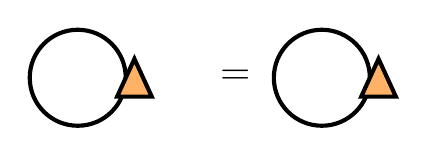
\begin{tikzpicture}
\draw[line width=1.5pt] (-2,0) circle (0.24in);
\draw[fill=orange!60, line width=1.5pt] (-1.5,-0.24) -- (-1.28,0.24) -- (-1.06,-0.24) -- cycle;
\node at (0,0) {\Large =};
\draw[line width=1.5pt] (1.1,0) circle (0.24in);
\draw[fill=orange!60, line width=1.5pt] (1.6,-0.24) -- (1.82,0.24) -- (2.04,-0.24) -- cycle;
\end{tikzpicture}
\vspace{0.35in}
\bigline{Is it the same?}\vspace{0.1in}
{\Large Yes.}
\end{center}
\pagenum{8}

% ============ PAGE 9 ============
\sprollpage
\begin{center}
\vspace*{0.8in}
\artnote{the ledger strip once more, alone, as if presented for a second try}
\ledgerCT
\vspace{0.35in}
\bigline{Let's follow it again.}
\end{center}
\pagenum{9}

% ============ PAGE 10 ============
\sprollpage
\begin{center}
\vspace*{0.7in}
\artnote{a completely fresh field, circle bold and chosen, exactly as before}

\begin{tikzpicture}
\draw[line width=3.5pt, fill=black!10] (-0.6,0) circle (0.28in);
\draw[line width=1.5pt, gray!40] (0.3,-0.28) rectangle (0.86,0.28);
\end{tikzpicture}
\vspace{0.3in}
\bigline{First: Pop the circle.}
\end{center}
\pagenum{10}

% ============ PAGE 11 ============
\sprollpage
\begin{center}
\vspace*{0.7in}
\artnote{the circle settled, triangle now bold and chosen}

\begin{tikzpicture}
\draw[line width=1.5pt] (-0.7,0) circle (0.28in);
\draw[fill=orange!60, line width=3.5pt] (0.4,-0.28) -- (0.68,0.28) -- (0.96,-0.28) -- cycle;
\end{tikzpicture}
\vspace{0.3in}
\bigline{Then: Pop the triangle.}
\end{center}
\pagenum{11}

% ============ PAGE 12 ============
\sprollpage
\begin{center}
\vspace*{0.7in}
\artnote{the circle and triangle together once more, identical to page 7}

\begin{tikzpicture}
\draw[line width=1.5pt] (-0.7,0) circle (0.28in);
\draw[fill=orange!60, line width=1.5pt] (0.4,-0.28) -- (0.68,0.28) -- (0.96,-0.28) -- cycle;
\end{tikzpicture}
\vspace{0.3in}
\bigline{Still the same.}
\end{center}
\pagenum{12}

% ============ PAGE 13 ============
\sprollpage
\begin{center}
\vspace*{0.6in}
\artnote{the ledger strip small in the corner, with three little copies of the circle-and-triangle result fanned out beside it, all identical}

\begin{tikzpicture}
\draw[line width=1pt, gray!50] (-2.2,0) circle (0.16in);
\draw[fill=orange!60, line width=1pt, gray!50] (-1.9,-0.16) -- (-1.75,0.16) -- (-1.6,-0.16) -- cycle;
\draw[line width=1pt, gray!50] (-0.2,0) circle (0.16in);
\draw[fill=orange!60, line width=1pt, gray!50] (0.1,-0.16) -- (0.25,0.16) -- (0.4,-0.16) -- cycle;
\draw[line width=1pt, gray!50] (1.8,0) circle (0.16in);
\draw[fill=orange!60, line width=1pt, gray!50] (2.1,-0.16) -- (2.25,0.16) -- (2.4,-0.16) -- cycle;
\end{tikzpicture}
\vspace{0.35in}
\bigline{Follow the same record.}\vspace{0.1in}
\bigline{Build the same thing.}\vspace{0.1in}
{\Huge \textbf{Every time.}}
\end{center}
\pagenum{13}

% ============ PAGE 14 ============
\sprollpage
\begin{center}
\vspace*{0.8in}
\artnote{a small open eye or magnifying glass beside the ledger strip, suggesting checking rather than guessing}
\ledgerCT
\vspace{0.35in}
\bigline{You don't have to guess.}\vspace{0.1in}
{\Large You can check.}
\end{center}
\pagenum{14}

% ============ PAGE 15 (closing / hand-off) ============
\sprollpage
\begin{center}
\vspace*{0.5in}
\artnote{the ledger strip, with a faint third line beneath it, empty except for a small shape drawn very lightly, almost a ghost, with a small line through it}
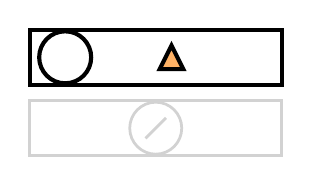
\begin{tikzpicture}
\draw[line width=1.5pt] (-1.6,0.55) rectangle (1.6,1.25);
\draw[line width=1.5pt] (-1.15,0.9) circle (0.13in);
\draw[fill=orange!60, line width=1.5pt] (0.05,0.75) -- (0.2,1.05) -- (0.35,0.75) -- cycle;
\draw[line width=1pt, gray!35] (-1.6,-0.35) rectangle (1.6,0.35);
\draw[line width=1pt, gray!35] (0,0) circle (0.13in);
\draw[line width=1pt, gray!35] (-0.13,-0.13) -- (0.13,0.13);
\end{tikzpicture}
\vspace{0.3in}
\bigline{But what if a record could say:}\vspace{0.1in}
{\Large not this way?}
\vspace{0.4in}\\
{\small \textit{--- turn the page for Sproll 04: Not This Way ---}}
\end{center}
\pagenum{15}

% ============ PAGE 16: Note for Grown-Ups (backmatter) ============
\sprollpage
\vspace*{0.3in}
{\large \textbf{A Note for Grown-Ups}}
\vspace{0.2in}

\normalsize
This book introduces replay: following a kept record, step by step, to rebuild what it describes, rather than only reading it. The record used throughout is the ledger strip introduced in Sproll 02.

\vspace{0.15in}
The claim this book asks a child to test for themselves, by literally doing it twice, is that a complete record, followed exactly, gives back the same result every time. This is not a simplification. It is the same guarantee that makes a recipe trustworthy or a set of instructions worth following, and it is given a precise formal treatment (a determinism proposition) in the technical companion material for this curriculum.

\vspace{0.15in}
Page 15 closes on a deliberately unresolved image: a faint, crossed-out shape in a third ledger line. This anticipates Sproll 04, which asks whether a record can describe something that was considered and specifically not chosen, and whether that is different from simply leaving it out of the record altogether.

\vspace{0.3in}
{\small Sproll 04: Not This Way continues directly from this book's final page.}
\pagenum{16}

\end{document}
